\documentclass[a4paper,10pt]{scrartcl}
\usepackage{physik-vorlesung}

\title{Experimentalphysik I}

\begin{document}

\maketitle

\tableofcontents

\newpage

\section*{Vorwort}
\begin{seg}{Ziele:}
\begin{itemize}
\item Experimentelle und theoretische Grundlagen der Newtonschen Mechanik, Wärmelehre, Thermodynamik
\item Als Einstieg möglichst auf sehr formale u. aufwendige Herleitungen verzichten, Grundprinzipien der Physik verdeutlichen
\item Veranschaulichung des Stoffs durch Demonstrationsexperimente in der Vorlesung
\item An physikalischen Beispielen werden die notwendige Bedingungen geklärt
\end{itemize}
\end{seg}

\begin{seg}{Ist Physik immer streng vorhersehbar?}
häufig ja, aber es gibt auch Ausnahmen:
\begin{itemize}
\item Wettervorhersage
\item \emph{chaotisches Pendel}
\item \emph{Galton-Brett}
\begin{figure}[h]
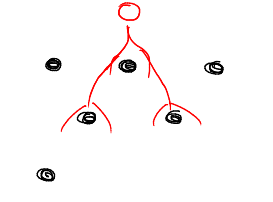
\includegraphics{fig1.png}
\end{figure}
\item \emph{Brownsche Bewegung}

\begin{figure}[h]
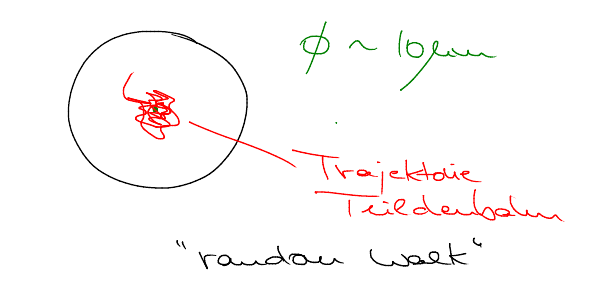
\includegraphics[scale=0.5]{fig2.png}
\end{figure}

\item \emph{Quantenmechanik}\\
Es gilt die Heisenbergsche Unschärferelation:
\[
\underbrace{\Delta x}_{\text{Ortsunschärfe}} \cdot \underbrace{\Delta p}_{\text{Impulsunschärfe}}
\]
\begin{figure}[h]
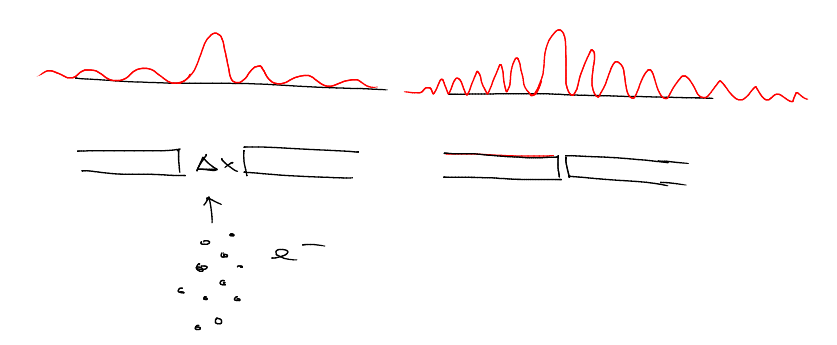
\includegraphics[scale=0.5]{fig3.png}
\end{figure}
\end{itemize}
\section{Physikalische Größen}
Eine \emph{Physikalische Größe} besteht aus einem \emph{Zahlenwert} und einer \emph{Einheit}.
\begin{ex*}
$1 \text{ in } \hat = \text{ Breite d. Daumens}$\\
Dies wurde später dann modifiziert, sodass die Einheit zur Länge drei aneinander liegenden Gerstenkörner umdefiniert worden ist.
\begin{figure}[h]
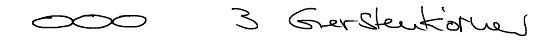
\includegraphics[scale=0.5]{fig4.png}
 \end{figure}
 
 Wünsche: wenige, aber überall nachprüfbare Einheiten $\rightarrow$ Basiseinheiten, Grundeinheiten
 \end{ex*}
 \end{seg}
 \subsection{Basiseinheiten}
 \begin{enumerate}[a)]
\item Zeit \\
Die Grundeinheit der Zeit ist $1$ Sekunde(s).  Diese lässt sich definieren durch den Vergleich mit periodischen Vorgang. Es gilt:
\[
\boxed{T=2\pi \sqrt{\frac{l}{g}}}
\]

\[
l=24,8 \text{cm} \rightarrow T=1s
\]
\begin{itemize}
\item Quarzplättchen besitzen eine Frequenz aus dem $kHz$-Bereich.
\begin{figure}[h]
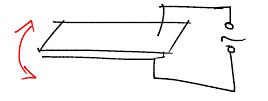
\includegraphics[scale=0.5]{fig5.png}
\end{figure}

Sie Besitzen einen Gangungenauigkeit von $1$ s/Woche. Sie besitzen also einen Fehler von $1$s pro $10^6$s
\item Es gibt aber auch die Möglichkeit mittels atomarer Eigenschwingungen (atomare Uhren) die Zeit noch genauer zu messen.  Deren Ganggenauigkeit entspricht $1$ s/$3000$ Jahren. Dies findet unter anderem Anwendung im GPS. 
\item $\ce{^{133}Cs}$ Hyperfeinübergang

Es ergibt sich die Definition $1\s=9.192.631.770$-faches der Periodendauer des Hyperfeinübergangs in $\ce{^{133}Cs}$. Diese ist überall nachvollziehbar!
\newpage
 \begin{seg}{Größenordungen von Zeiten}
 
 \begin{center}
% \begin{table}[h]
 \begin{tabular}{l r}
 Weltall: & $10^8 \s$ \\
 Mensch: & 1$10^9 s$ \\
 Pulsschlag: & $1 s$ \\
 Licht durchläuft $30 cm$: & $10^-9 s$ \\
 Licht durchläuft Atom: & $10^-18 s$
 \end{tabular}
% \end{table}
 \end{center}
 \end{seg} 
Mit Hilfe von Präfixen kann man den Einheit eine neue Größenordnung geben. Hier die geläufigen Präfixe:

\begin{center}
% \begin{table}[h]
 \begin{tabular}{l c r}
  $1\m$ & Milli & $10^{-3}$\\
  $1\my$ & Mikro & $ 10^{-6}$\\
 $1\n$ & Nano & $ 10^{-9}$ \\
 $1\p$ & Piko & $ 10^{-12}$\\
 $1\f$ & Fakto & $10^{-15}$\\
 $1\a$ & Atte & $10^{-18}$\\
 $1\k$ & Kilo & $10^3$ \\
 $1\M$ & Mega & $10^6$ \\
 $1\G$ & Giga & $10^9$ \\
 $1\T$ & Terra & $10^12$ \\
 $1\P$ & Peta & $10^15$ \\
 $1\E$ & Exa & $10^18$
 \end{tabular}
% \end{table}
\end{center}

 
 Zeitmessung durch radioaktiven Zerfall Kerne mit großer Masse $\rightarrow$ instabil $N=$ Zahl instabiler Kerne. \\
 charakteristisch: $\frac{dN}{dt} ~ N(t)$
 Wahrscheinlich, dass Kern zerfällt ist unabhänfig von allem anderen Kernen.
 \begin{equation}
  \frac{dN}{dt}=-\lambda \cdot N(t), \qquad \lambda: \text{ Zerfallskonstanste}, \lambda>0
 \end{equation}
 \begin{equation}
  N(T)=N_0 \cdot e^{-\lambda t}, \qquad N_0:= N(0), [\lambda]=\frac{1}{s}
 \end{equation}

 \begin{figure}[h]
  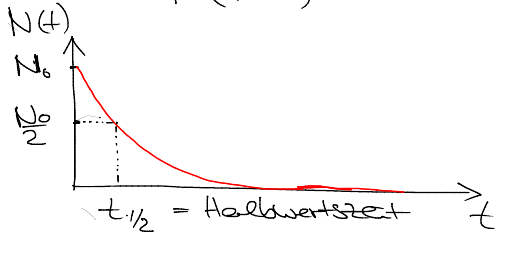
\includegraphics[scale=0.5]{fig6.png}
 \end{figure}

\begin{align*}
  \frac{N_0}{2} &= N_0 \cdot e^{-\lambda t_{\frac 1 2}}\\
  \ln 0.5 &=-\lambda \cdot t_{\frac 1 2} \\
  t_{\frac 1 2} &= - \frac{\ln 0.5}\lambda = {\ln 2}{\lambda} 
\end{align*}

 \begin{ex*}
  \begin{enumerate}[a)]
   \item $\ce{^{224}_{88} Tn} \rightarrow \ce{^{220}_{86} Ru} + \alpha, \qquad \alpha=\ce{^4_2 He}$ mit Halbwertszeit $t_{\frac 1 2}=556s$
   \item $\beta$-Zerfall: $\ce{^{14}_6 C} \to \ce{^{14}_7 N} + e^- \bar v_l$ mit Halbwertszeit $t_{\frac 1 2}=5730 a$  
 \end{enumerate}
 \end{ex*}
 
 
\item Radio-Carbon-Methode \\
 Kohlenstoff: $\ce{^{12}_6 C}, \ce{^{13}_6 C}, \ce{^{14}_6 C}$

 Verteilung in Atmosphäre

 \begin{align*}
  \ce{^{12} C}:  98,89\% \\
  \ce{^{13} C}: 1,11\% \\
 \ce{^{14} C}: 10^-10 \% \\
 \end{align*}
 Wobei erstere beiden stabil und $\ce{^{14} C}$ instabil ist.  Lebende Organismen besitzen aufgrund von Stoffaustausch identische Kohlenstoff-Verteilung.  Stirbt der Organismus verändert sich das Isotopenverhältnis.

 
 \begin{align*}
  \ce{^{14} C(t)}&=\ce{^{14} C_0} \cdot e^{-\lambda t} \\
 \ce{^{13} C(t)}&=\ce{^{12} C_0}\\
 \frac{\ce{^{14} C}}{\ce{^{12} C}} |_\text{Fossil} (t)&= \frac{\ce{^{14} C_0}}{\ce{^{12} C_0}} e^{-\lambda t}, \qquad \lambda=1.121\cdot 10^{-4} \frac{1}{a}
 \end{align*}
 \item C14-Methode: experimentelle Bestimmung\\
 $\frac{\ce{^{14}  C}}{\ce{^{12} C}}$ im Fossil (Massenspektrum) $\rightarrow$ Alter $t \rightarrow$ Alter + Höhlenzeichnung in S-Frankreich:  $15.500$ Jahre
 \end{itemize} 
 \item Länge

 1799: $1 \m \hat = \frac{1}{400000000}$ des durch Paris gehenden Großkreises ($40\cdot 10^3$ km). Dadurch ergab sich die Grundeinheit $1$m.

 Urmeter: $\ce{Pt_{90}}$ $\ce{Ir_{10}}$

 Seit 1983:
 \[
  1\m=\text{ Länge des Weges Weges, den Licht im Vakuum in $\frac{1}{299792485} s$ zurücklegt.}
 \]

\begin{seg}{Größenordnungen und Längen}


 \begin{tabular}{l r}
  Fixstern & $4\cdot 10^16 \m$\\
  Erde-Sonne & $1.5 \cdot 10^11 \m$\\
 Erdradius & $63 \cdot 10^6 \m $\\
 Sichtbares Licht (Wellenlänge) & $ 500\cdot 10^-9$m \\
 Atomdurchmesser & $10^-10$m  \\
 Kerndurchmesser & $10 ^-15$m
 \end{tabular}
 \end{seg}
 \begin{seg}{Messung von Abständen}
 Triangulation:
 \begin{figure}[h]
  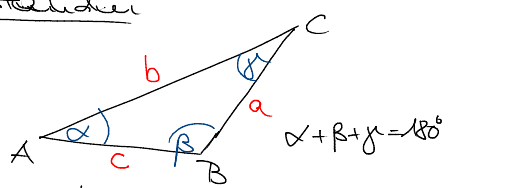
\includegraphics[scale=0.5]{fig7.png}
 \end{figure}
 Sinussatz: $\frac{c}{\sin\gamma} = \frac{a}{\sin{\beta}}=\frac{a}{\sin\alpha}$ \\
 
 \begin{itemize}
  \item $\alpha, \beta$ bekannt $\to \gamma$ bekannt
  \item $c$ bekannt, dann lässt sich $a$ bzw. $b$ berechnen zu:
\begin{align*}
a&=c\cdot \frac{\sin \alpha}{\sin \gamma}\\
b&=c\cdot \frac{\sin \beta}{\sin \gamma}
\end{align*}
 \end{itemize}
\end{seg}
 \begin{seg}{Abstand-Erde-Mond}
 \begin{figure}[h]
  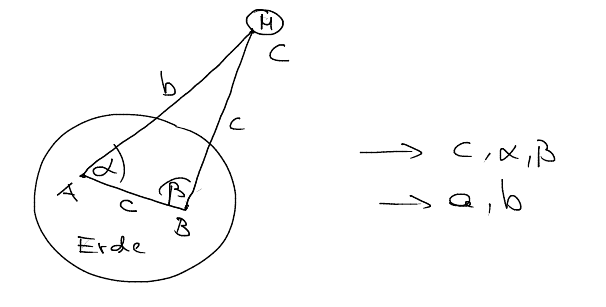
\includegraphics[scale=0.5]{fig8.png}
 \end{figure}
\end{seg}
 \begin{seg}{Abstand Erde-Sonne}
 Als Basis (c) wähle Erde-Mond
 \begin{figure}[h]
  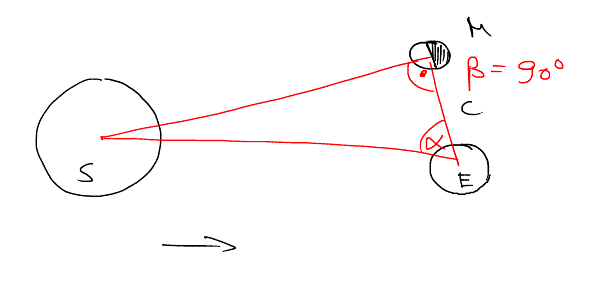
\includegraphics[scale=0.5]{fig9.png}
 \end{figure}
 Bei Halbmond besitzt $\beta=90^\circ$.  Den Abstand Erde-Mond lässt sich messen. Dann genügt es Den Winkel zwischen Mond und Sonne auf der Erde messen und damit ergibt sich der Abstand zum Mond.
 \end{seg}
 \begin{seg}{LIDAR (Light Detection and raging)}
 \begin{figure}[h]
  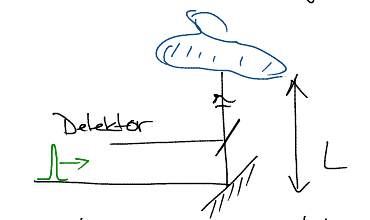
\includegraphics{fig10.png}
 \end{figure}
 \[
 T=\frac{2L}{c}
 \]
\end{seg}
 \begin{seg}{Messungen kleiner Entfernungen Laserinterferometer (\emph{Michelson-Interferometer})}

 \begin{figure}[h]
  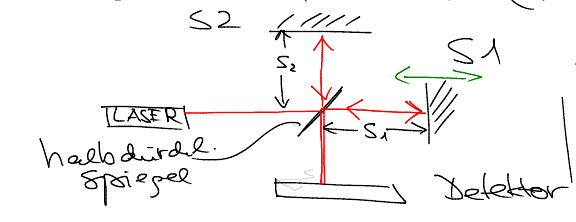
\includegraphics[scale=0.7]{fig11.png}
 \end{figure}

 \[
  \Delta s= 2 |s_1-s_2|
 \]

 Die Verschiebung um $\frac{20 \my m}{\text{64 Maxima}}=0.625 \to \lambda=630\my \m $
\end{seg}
 \item Masse \\
 Die Grundeinheit ist $1kg \hat = \text{Masse des Urkilogramms Zylinder/ } \ce{Pt_{90}}\ce{Ti_{10}}$

 Vermutlich 2014:

 \[
  1 \txt{Mol}= 6022\cdot 10^{23} \cdot \ce{^{28} Si} \hat = 28.09 g
 \]
 \[
 35,599 \,\text{Mol}\, \ce{^{28} Cr} \hat = 1 \kg
 \]
 \[
 2,1441 \cdot 10^{25} \ce{^{28} Si} \text{Atome} \hat = 1 \kg
 \]

 Zeit, Länge, Masse sind die Grundgrößen der Kinematik, die zugehörigen Standardeinheiten bilden das \emph{SI}.
\end{enumerate}
\subsection{Messfehler}
\begin{enumerate}[a)]
\item Systematische Messfehler
\begin{itemize}
\item falsch geeichtes Messinstrument
\item Nichtberücksichtigen von \emph{Konstanten} äußerer Einflüsse
\item Näherungsformeln außerhalb Gültigkeitsbereich (für kleine Winkel $\alpha$ gilt zum Beispiel $\sin \alpha \approx \alpha$ und $\cos \alpha \approx 1$
\end{itemize}
$\implies$ Systematische Messfehler verfälschen Messergebnis um gleichen Betrag und Richtung \\
$\rightarrow$ sie sind also prinzipiell vermeidbar
\item statistische zufällige Messfehler
\begin{itemize}
\item[$\rightarrow$] Können Messergebnis in beide Richtungen verändern.
\item Beobachter selbst 
\item statistische Änderungen äußerer Einflüsse
\item[$\rightarrow$] Die Messwerte streuen daher um einen bestimmten Wert
\item[$\rightarrow$] nicht vermeidbar aber durch wiederholte Messung verringerbar
\end{itemize} 
\end{enumerate}
\begin{seg}{Bildung des arithmetischen Mittels}
Sei unsere Messreihe $x_1, x_2, x_3, ..., x_n$, wobei $n$ die Zahl unserer Messungen darstellt, so ergibt sich das arithmetische Mittel durch:
\[
\boxed{\bar x = \frac{x_1+x_2+x_3+...+x_n}n=\frac{1}{n} \sum_{i=1}^{n} x_i}
\]
Je mehr Messungen gemacht werden, desto genauer entspricht $\bar x$ dem empirischen Mittelwert.  Die \emph{Standardabweichung} $\sigma$ (\emph{Streuung}) gibt an, wie zuverlässig Einzelmessungen sind.
\begin{figure}[h]
%\includegraphics{fig12.png}
\end{figure}
\[
\boxed{\sigma=\sqrt{\frac 1 {n-1} \sum\limits_{i=1}^n (x_i-\bar x)^2}}
\]
Häufig kommt es zur \emph{Gaußverteilung} der Messwerte: Es ergibt sich die Dichtefunktion:
\[
\boxed{p(x)=\frac{1}{\sqrt{2\pi}\cdot \sigma} \cdot e^{-\frac{(x-\bar x)^2}{2\sigma^2}}}
\]
\begin{figure}[h]
%\includegraphics{fig13.png}
\end{figure}
Als Dichtefunktion besitzt $p$ die Eigenschaft: 
\[
\int\limits_{-\infty}^{+\infty}p(x) dx = 1
\]
Die Wahrscheinlichkeit $P$, das x im Intervall $\bar x \pm \sigma$ streut ist damit. 
\[
\int\limits_{\bar x-\sigma}^{\bar x+\sigma} p(x)=0,683
\]
Man bezeichnet dies auch als \emph{statistische Sicherheit} bzw. \emph{Vertrauensgrenze} $P$ für $\delta=\sigma$.

\begin{seg}{Statistische Sicherheit bzw. Vertrauengrenze $P$ für $\delta$}
\begin{table}[h]
\begin{tabular}{c|c}
$\delta[\sigma]$ & $P=\int\limits_{\bar x-\delta}^{\bar x+\delta} p(x) dx$ \\ \hline
1 & 0,683 \\
0,676 & 0,5 \\
1,96 & 0,95 \\
3,0 & 0,997
\end{tabular}
\end{table}
\end{seg}
\end{seg}
\section{Kinematik}
\subsection{Eindimensionale Bewegung}
\begin{enumerate}[a)]
\item gleichförmige Bewegung ($\vec v=\text{const.}$)

\begin{seg}{Weg-Zeit-Diagramm für $\vec v=6\frac{\m}{\s}$}
\begin{figure}[h]
%\includegraphics{fig14.png}
\end{figure}
\end{seg}
Es gilt:
\[
\boxed{\vec v=\frac{\Delta s}{\Delta t} \left (\frac{\m}{\s}\right )}
\]
$\vec v$ ist die Steigung des Weg-Zeit-Diagramms.
\item Nicht-Gleichförmige Bewegung ($\vec v\neq \txt{const.}$)
\begin{figure}[h]
%\includegraphics{fig15.png}
\end{figure}
Die \emph{mittlere Geschwindigkeit} ergibt sich zu:
\[\boxed{\bar v=\frac{\Delta s}{\Delta t}}\]
Die \emph{Momentangeschwindigkeit} entspricht:
\[\boxed{\vec v=\lim\limits_{\Delta t \rightarrow 0} \frac{\Delta s}{\Delta t}= \frac{ds}{dt}}\]
Die Momentangeschwindigkeit $\vec v$ entspricht also der Steigung der Tangente zum Zeitpunkt $t=t_0$. Ist Die Momentangeschwindigkeit nicht konstant, so handelt es sich um eine \emph{beschleunigte} Bewegung.  Die \emph{Beschleunigung} ist für konstante Beschleunigungen gegeben durch:
\[
\boxed{a=\frac{\Delta v}{\Delta t}}
\] 
$a=\txt{const.}$:
\begin{figure}[h]
%\includegraphics{fig16.png}
\end{figure}
$a\neq\txt{const.}$:
\begin{figure}[h]
%\includegraphics{fig17.png}
\end{figure}

Die \emph{Momentanbeschleunigung} ergibt sich zu:
\[
\boxed{a(t)=\lim\limits_{\Delta t \rightarrow 0} \frac{\Delta v}{\Delta t}=\frac{dv}{dt}=\frac{d^2s}{dt^2}\left [\frac{\m}{\s^2}\right ]}
\]
\begin{seg}{Bestimmung von $v(t)$ und $s(t)$}
Es gilt $\frac{dv(t)}{dt}=a(t)$.  Nach integrieren der Gleichung ergibt sich:
\[
\int\limits_0^t \frac{dv(t')}{dt'}dt'=v(t)-v_0=\int\limits_0^t a(t')dt'
\]
wobei $v_0:=v(0)$.  Für $a(t)=a_0=\txt{const.}$ ergibt sich:
\[
\boxed{v(t)=a_0\cdot t+v_0}
\]
Es ist $\frac{ds}{dt}=v$ und es ergibt sich analog:
\begin{align*}
s(t)-s_0&=\int\limits_0^t v(t')dt', s_0:= s(0)\\
s(t)    &=\int\limits_0^t (a_0\cdot t'+v_0)dt'+s_0
\end{align*}
und letztlich ergibt sich:
\[
\boxed{s(t)=\frac{1}{2}a_0t^2+v_0t+s_0}
\]
\end{seg}
\begin{seg}{graphische Darstellung}
\begin{figure}[h]
%\includegraphics{fig18.png}
\end{figure}
Wir können den Weg aus der Beschleunigung bestimmen:
\[
\iint a \,dt\, dt\stackrel{a\approx a_0}{=}\int a_0\cdot t \,dt=\frac{1}{2}a_0t^2=s
\]
\end{seg}
\end{enumerate}
\subsection{Räumliche Bewegung}
Wir können einen Übergang zu vektoriellen Größen Herstellen.  
\begin{figure}[h]
%\includegraphics{fig19.png}
\end{figure}
Wir bezeichnen $\vec r$ als \emph{Ortsvektor} von $P$.  Der Betrag des Vektors ist gegeben durch: $|\vec r|=\sqrt{x_0^2+y_0^2}$.
Wir benutzen die Schreibweise $\vec r=(x_0,y_0)$.  Mögliche Notationen zur Darstellung von Vektoren sind: $\vec r, \stackrel\rightharpoonup r, \underline{r}$.  Für 3-dimensionale Vektoren verwenden wir die Darstellung \[\vec r=\begin{pmatrix} r_x\\ r_y\\r_z \end{pmatrix}; \vec r= \begin{pmatrix} x\\ y\\z \end{pmatrix}\]
\begin{seg}{Addition von Vektoren}
Wir addieren Vektoren komponentenweise:
\[
\vec a+ \vec b=\begin{pmatrix} a_x+b_x\\ a_y+b_y\\a_z+b_z \end{pmatrix}
\]
\begin{figure}[h]
%\includegraphics{fig19.png}
\end{figure}
\end{seg}
\begin{seg}{Subtraktion von Vektoren}
Wir subtrahieren Vektoren komponentenweise:
\[
\vec a- \vec b=\begin{pmatrix} a_x-b_x\\ a_y-b_y\\a_z-b_z \end{pmatrix}
\]
\begin{figure}[h]
%\includegraphics{fig20.png}
\end{figure}
Beschreibung von Vektoren ist abhängig vom Koordinatensystem:
\end{seg}

\begin{seg}{Kartesisches Koordinatensystem (rechtwinklig, rechtshändig}
\begin{figure}[h]
%\includegraphics{fig21.png}
\end{figure}[h]
\begin{figure}[h]
%\includegraphics{fig22.png}
\end{figure}
$r(t)$ ist ein zeitabhängiger Ortsvektor und beschreibt dadurch eine Ortskurve. Die Notation:
\[
\vec r(t)=\begin{pmatrix} x(t)\\ y(t)\\z(t) \end{pmatrix}
\]
Alternativ ist auch denkbar:
\begin{align*}
\vec r(t)&=(x(t),y(t),z(t))\\
\vec r(t)&=x(t)\cdot \vec e_x+y(t)\cdot \vec e_y+z(t)\cdot\vec e_z
\end{align*}
wobei $\vec e_x, \vec e_y, \vec e_z$ die Einheitsvektoren der Koordinatenachsen sind. Der Betrag des Vektor ergibt sich zu:
\[
r(t)=|\vec r|=\sqrt{{x(t)}^2+{y(t)}^2+{z(t)}^2}
\]
\end{seg}
Wir erinnern uns an die Definition für die Geschwindigkeit für eindimensionale Bewegungen:
\begin{align*}
v&=\frac{ds}{dt}\\
a&= \frac{dv}{dt}=\frac{d^2s}{dt^2}
\end{align*}
f+r $a=a_0=\txt{const.}$ ergab sich:
\begin{align*}
v(t)&=a_0\cdot t+v_0, v_0=v(0)\\
s(t)&= \frac{1}{2} a_0t^2+v_0\cdot t+s_0, s_0=s(0)
\end{align*}
Betrachten wir also eine Bewegung, die durch eine Ortskurve gegeben ist.
\begin{figure}[h]
%\includegraphics{fig23.png}
\end{figure}
Sei $\Delta r=r(t+\Delta t)-r(t)$ Für $\Delta t\rightarrow 0$ gilt $\Delta s\approx \Delta r$.  Folgende Definitionen für Geschwindigkeit und Beschleunigung sind daher naheliegend:
\begin{df}[Geschwindigkeit]
Die Geschwindigkeit $\vec v(t)$ ist definiert durch:
\[\vec v(t)=\lim\limits_{\Delta t\rightarrow 0} \frac{\Delta \vec r}{\Delta t} = \frac{d\vec{r}}{dt}=\dot{\vec r}=(\frac{dx}{dt},\frac{dy}{dt},\frac{dz}{dt})=(v_x(t),v_y(t),v_z(t))\]
Hierbei zeigt $\vec v(t)$ in Richtung der Bahntangente an die Ortskurve $\vec r(t)$.
\end{df}
\begin{df}[Beschleunigung]
Die Beschleunigung $\vec v(t)$ ist definiert durch:
\[\vec a(t)=\lim\limits_{\Delta t\rightarrow 0} \frac{\Delta \vec v}{\Delta t} = \frac{d\vec{v}}{dt}=\frac{d^2\vec{v}}{dt^2}=\ddot{\vec r}=(\frac{d^2x}{dt^2},\frac{d^2y}{dt^2},\frac{d^2z}{dt^2})=(a_x(t),a_y(t),a_z(t))\]
\end{df}
Wir betrachten nun die Beschleunigung zur Bahn eines Massenpunkts.  Diese ist im Allgemeinen nicht mit der Bahntangenten identitisch. $\vec a$ kann sowohl eine Tangentialkomponente wie auch eine Normalkomponente besitzen. Wir bezeichnen in Folge den Einheitsvektor tangential zur Bahnkurve mit $\vec u_T$.
\[
\boxed{\vec a=\frac{d\vec{v}}{dt}=\frac{d}{dt}(|\vec v|\cdot \vec u_T)=\underbrace{\frac{d|\vec v|}{dt}\cdot\vec u_T}_{\txt{\tiny{Tangentialkomponente}}}+\underbrace{|\vec v|\cdot \frac{d\vec{u_T}}{dt}}_{\txt{\tiny{Normalkomponente}}}} 
\]
\begin{enumerate}
\item geradlinige Bahn des Massenpunktes
\begin{figure}[h]
%\includegraphics{fig24.png}
\end{figure}
$\vec u_T$ zeigt immer in gleiche Richtung und damit ist $\frac{d\vec{u_T}}{dt}=0$ und
\[
\boxed{\vec a=\frac{d|\vec v|}{dt}\cdot {\vec{u_T}}}
\]
$\vec v$ und $\vec a$ besitzen gleiche Richtung.
\item betrachten wir eine gekrümmte Bahn so ist $\frac{d\vec{u_T}}{dt}\neq 0$
\begin{figure}[h]
%\includegraphics{fig25.png}
\end{figure}
Unter Ausnützung der Ähnlichkeit der beiden Dreiecke ergibt sich bei einer Kreisbahn gerade:
\[
\frac{|\Delta \vec u_T|}{|\vec u_T|}=\frac{\Delta s}{R}\implies |\Delta \vec u_T|=\frac{1}{R}\cdot \Delta s
\]
nach dem Differenzieren auf beiden Seiten (Überlegen Sie sich, warum sie dies so machen dürfen!):
\[
|\frac{d\vec{u_T}}{dt}|=\frac{1}{R}\cdot |\vec v|
\]
Die Normalkomponente steht dabei gerade orthogonal zum Tangentialkomponente der Beschleunigung (Übung!), denn es gilt $\frac{d\vec{u_T}}{dt}\perp   \vec u_T$ (Übung!), dies ist gerade dann der Fall, wenn $\alpha \rightarrow 0$. Man sagt $\frac{d\vec{u_T}}{dt}$ steht "`normal"' zur Bahnkurve.
\begin{figure}[h]
%\includegraphics{fig26.png}
\end{figure}
Es ergibt sich für die Beschleunigung:
\[
\va=\frac{d|\v|}{dt} \cdot \u_T+\vec{u_N}\cdot \frac{d\u_T}{dt}=\underbrace{\frac{d|\v|}{dt}}_{a_T} \cdot \u_T+\underbrace{\frac{|\v|^2}{R}}_{a_N}\cdot \vec{u_N}
\]
Der Betrag von $\va$ ergibt sich zu: $|\va|=\sqrt{a_T^2+a_N^2}=\sqrt{\left (\frac{d|\v|}{dt}\right )^2+\left ( \frac{v^2}R \right )^2}$
\end{enumerate}
\begin{ex*} Wir betrachten zwei Spezialfälle
\begin{enumerate}[a)]
\item geradlinige Bewegung
\[
R\rightarrow \infty \implies a_N\rightarrow 0
\] 
\item $|\v|=\txt{const.} \implies a_T=0$, aber $a_N\neq 0$. Es handelt sich hierbei um eine Kreisbewegung. 
\end{enumerate}
\end{ex*}
Es gilt das \emph{Superpositionsprinzip:}

\begin{seg}{Superpositionsprinzip:} Wenn ein Körper mehrere Bewegungen in verschiedenen Richtungen gleichzeitig ausführt, dann sind die Bewegungen in jeder Richtung unabhängig von den Bewegungen in den anderen Richtungen. 
\end{seg}
\begin{seg}{lineare Überlagerung von Bewegun in unterschiedliche Raumrichtungen}
\begin{itemize}
\item \emph{horizontaler Wurf}\\
Beim horizontalen Wurf komm es zu einer Überlagerung von konstanter horizontaler Geschwindigkeit $v_{x_0}$ und freien Fall.
\begin{align*}
x&=v_{x_0}\cdot t\\
y&=-\frac 1 2 \underbrace{g}_{\approx 10\frac{\m}{\s^2}}t^2
\end{align*}
\begin{figure}[h]
%\includegraphics{fig27.png}
\end{figure}
\[
t=\frac{x}{v_{x_0}} \implies \boxed{y=-\frac{1}{2} g \frac{x^2}{v_{x_0}^2}}
\]
Damit besitzt die Ortskurve eine Parabelbahn. Ihr Maximum nimmt sie gerade im Ursprung an.
\item \emph{Schiefer Wurf}\\
Beim schiefen Wurf kommt es zur Überlagerung von konstanter Geschwindigkeit in beliebiger Richtung und dem freien Fall. Zunächst lässt sich $\vec v_0$ in Horizontal- und Vertikalkomponente aufspalten:
\[
\v_0=\v_{0x}+\v_{0y}
\]
Für die Komponenten ergibt sich in Abhängigkeit zur Zeit $t$:
\begin{align*}
x&=v_{x_0}\cdot t\\
y&=v_{y_0}\cdot t-\frac{1}{2}gt^2
\end{align*}
\begin{figure}[h]
%\includegraphics{fig28.png}
\end{figure}
Es ergibt sich die Parabelbahn:
\[
\boxed{y=v_{y_0}\cdot \frac{x}{v_{x_0}}-\frac 1 2 g \frac{x^2}{v_{x_0}^2}}
\]
\item \emph{Kreisbewegung}\\
Bei der Kreisbewegung gilt:
\begin{align*}
x&=R\cdot\cos{\phi}\\
y&=R\cdot\sin{\phi}
\end{align*}
Für $\frac{d\phi}{dt}=\txt{const.}$ ergibt sich eine gleichförmige Kreisbewegung, der Betrag der Geschwindigkeit ist konstant.  
\begin{df}[Winkelgeschwindigkeit]
Die Winkelgeschwindigkeit $\omega$ ist definiert durch:
\[
\omega =\frac{d\phi}{dt}
\]
Entsprechend gilt $v=\frac{ds}{dt}$.
\end{df}
Die Einheit von $\omega$ ist $\frac{\txt{rad}}{\s}$ bzw. $\frac 1 \s$
\end{itemize}
\begin{seg}{Exkurs: Winkelmessung}
Es gibt zwei Möglichkeiten Winkelgrößen zu definieren, entweder in dem man $1$° als Teil eines Vollkreises.
\[
1^\circ \hat = \frac{1}{360} \txt{Vollkreis}
\]
oder über die Bogenlänge am Einheitskreis (also als \emph{Radiant}). Charakteristische Größen sind:
\begin{align*}
360°&=2\pi=6,28 \rad\\
1 \rad &\approx 57,29°\\
1°&\approx 0,0017 \rad
\end{align*}
$\rad$ ist eine dimensionslose Größe.
\end{seg}
$\omega$ ist ein Vektor mit Betrag $|\omega|=\frac{d\phi}{dt}$ orthogonal zur Kreisebene gerichtet.
\begin{figure}[h]
%\includegraphics{fig29.png}
\end{figure}
Die Richtung von $\omega$ bestimmt sich mittels der \emph{rechte-Hand-Regel}:
\begin{figure}[h]
%\includegraphics{fig30.png}
\end{figure}
Für den Winkel gilt also bei einer gleichförmigen Kreisbewegung:
\[
\phi(t)=\omega\cdot t
\]
bzw. für die Komponenten:
\begin{align*}
x&=R\cdot \cos(\omega t)\\
y&=R\cdot \sin(\omega t)
\end{align*}
Für die \emph{Periodendauer} $T$ (Zeit für einen Umlauf) ergibt sich $T=\frac{2\pi}{\omega}$. Für die \emph{Frequenz} $\nu$ (Zahl der Umläufe pro Sekunde) ergibt sich $\nu=\frac{1}{T}=\frac{\w}{2\pi}$. Die Geschwindigkeit des Massenpunktes P auf der Kreisbahn ist bestimmt zu $|\v|=\frac{2\pi\cdot R}{T} \hat=\frac{\txt{Strecke}}{\txt{Umlaufzeit}}$ und damit $|\v|=\omega \cdot R$.

Für $\omega=\txt{const.}$ ist auch $|v|=\const$, aber die Richtung von $\vec v$ ändert sich, da sie tangential zur Bahnkurve gerichtet ist. 
\end{seg}
\fixme[Vorlesung 5 und 6 fehlen]\\
\fixme[Bild fehlt]\\
\begin{itemize}
 \item 
\begin{seg}{Zentripetalkraft}
\fixme[Bild fehlt]\\
\begin{align*}
 |\vec a|&=\omega^2\cdot R\\
F&=m\omega^2\cdot R\\
\omega&=\frac{v}{R}, F=\frac{mv^2}{R}
\end{align*}
\end{seg}
\item 
\begin{seg}{Federkraft}
 \fixme[Bild fehlt]\\
Diese Gesetzmäßigkeit nennt man das \emph{Hooksche Gesetz}. Man bezeichnet $D$ als Federkonstante.
\end{seg}
\end{itemize}
\subsection{Scheinkräfte}
Bisher haben wir noch kein Bezugssysteme fesgelegt. Dies möchten wir nun tun.
\begin{df}[Inertialsystem]
 Ein \emph{Inertialsystem} ist ein Bezugssystem für das, das II. Netwonsche Axiom gilt ($F=ma$)
\end{df}
Bei einem beschleunigten Bezugssystem scheinen die Newtonsche Axiome verletzt zu sein. Es entstehen sogenannte \emph{Scheinkräfte}
\subsubsection{geradlinige beschleunigte Bewegung}
\begin{enumerate}[a)]
 \item \fixme[Bild fehlt]\\
\begin{seg}{Ruhender Betrachter}
ein Beobachter, der relativ ruhend zum System, in dem sich der Wagen bewegt, sich befindet.
\underline{Der Körper bleibt in Ruhe}. Dies ist klar, da keine Kraft auf Körper wirkt.
\end{seg}
\begin{seg}{Mitbewegter Beobachter}
 Körper bewegt sich nach links. Eine Kraft muss auf den Körper wirken.
\end{seg}
Es kommt zu einer so genannten \emph{Scheinkraft} $\vec F_s=-m\cdot \va=-\vec F$.
\item \fixme[Bild fehlt]
Bei Beschleunigung wird Feder zunächst etwas zusammengedrückt. Zunächst etwas zusammengedrückt und bleibt, dann in diesem konstant. Spannungszustand.
\begin{seg}{Ruhender Beobachter}
 Körper bewegt sich mit $\va$ nach rechts. Es gilt $\vec F=m\cdot \va$. Die Ursache der Kraft $\vec F$ ist klar.\\
\fixme[Bild fehlt]
\end{seg}
\begin{seg}{Beschleunigter Beobachter}
 Körper bleibt in Ruhe. Also gilt für die Kraft $F\stackrel{!}{=}0$. Die Federkraft muss durch weitere Kraft kompensiert werden.
\[
 \vec F_D+\vec F_S=0
\]
\fixme[Bild fehlt]
\end{seg}
Generell gilt: Scheinkräfte mussen eingeführt werden, wenn Messungen in beschleunigten Bezugssystemen durchgeführt werden.
(In Inertialsystemen existieren dagegen keine Scheinkräfte.)
\begin{ex*}[Maxwellsches Rad]
\fixme[Bild fehlt]
Sowohl bei Abwärts- als auch bei Aufwärstsbewegung ergibt sich eine scheinbar \underline{kleinere} Masse.
\end{ex*}
\begin{att*}
 Beschleunigung zeigt in beiden Fällen nach unten
\end{att*}
\subsubsection{Scheinkräfte in rotierenden Bezugssystemen}
\begin{ex*}
 \fixme[Bild fehlt]
\begin{seg}{Ruhender Beobachter $S'$}
 $S'$ beobachtet eine geradlinige, gleichförmige Bewegung des Objekts, da $\vec F=0$
\end{seg}
 \begin{seg}{Mitbewegter Beobachter $S$}
  Objekt scheint von fiktiver Kraft vom Waggon geschleudert zu werden. 
 \end{seg}
\end{ex*}
Wir bezeichnen das ruhende Bezugssystem mit $S'(x',y',z')$ (grün) und das rotierende Bezugssystem mit $S(x,y,z)$.
Ein Spezialfall stellt beispielsweise die Rotation mit $\w$ um die $z$-Achse 
\\ \fixme[Bild fehlt]\\
Ein Körper der Masse $m$ bewege sich in $S'$ auf Trajektorie:
\[
 \vec r'(t)=x'(t)\cdot \vec{e_x}'+y'(t)\cdot \vec{e_y}'+z'(t)\cdot \vec{e_z}
\]
Wir beschreiben die identische Bahn von $S$ nun auf $\vec r'(t)=\vec r(t)$:
\begin{align*}
 \vec r'(x)&=\vec r(x)=x(t)\cdot \vec{e_x}+y(t)\cdot \vec{e_y}+z(t)\cdot \vec{e_z}\\
\frac{d\vec r'}{dt}&=\frac{d\vec r}{dt}=\underbrace{\left ( \frac{dx}{dt}\cdot \vec{e_x}+\frac{dy}{dt}\cdot \vec{e_y}+\frac{dz}{dt}\cdot \vec{e_z}\right )}_{
\text{\tiny{Geschwindigkeit im rotierenden Bezugssystem}}}+\underbrace{\left (\frac{d\vec{e_x}}{dt}\, x+\frac{d\vec{e_y}}{dt}\,y+\frac{d\vec{e_z}}{dt}\,z \right )}_{\text{\tiny{Rotation, der EInheitsvektoren von $S'$ aus betrachtet}}}
\end{align*}
\begin{seg}{Zeitliche Ableitung eines Vektors}
 \fixme[Bild fehlt]
%   \begin{align*}
%    |d\vec{u}|&=d\phi\cdot u_\perp\\
%    |\frac{d\vec{u}}{dt}|&=\frac{dy}{dt}\cdot \vec{e_y}+\frac{dz}{dt}\cdot \vec{e_z}\right )\frac{d\phi}{dt}\cdot u_\perp=|\w|\cdot u_\perp
%   \end{align*}
Es ist $\vec u \cdot \sin\gamma=u_\perp$:
\[
 |\frac{d\vec{u}}{dt}|=|\w|\cdot |\vec u|\cdot \sin \gamma
\]
Die Richtung von $\frac{d\vec{u}}{dt}$, ist gerade orthogonal zu $\vec{\w}, \vec u )$ (für $d\phi\rightarrow 0$).
Daraus ergibt sich 
\[
 \boxed{\frac{d\vec{u}}{dt}=\w\times \va}=w\cdot u \cdot \sin \gamma
\]
\end{seg}
\begin{seg}{Spezialfall} 
$S'(x',y',z')$ ist ruhend und $S(x,y,z)$ toriert mit $\omega$ um die $z$-Achse. Ruhe der Massepunkt in $S'$. Also gilt $v'=0$.
\end{seg} 
\begin{seg}{Frage}
Wie sieht Bewegun von $S$ betrachtet aus?
\end{seg}
\fixme[Bild fehlt]\\
(Der Ortsvektor ergibt sich unabhängig von Bezugssystem).
\[
 \frac{d\vec{r'}}{dt}=\frac{d\vec r}{dt}=0=\underbrace{\v}_{\text{\tiny{Geschwindigkeit in $S$}}}+
\underbrace{\frac{d\vec{e_x}}{dt}x+\frac{d\vec{e_y}}{dt}y+\frac{d\vec{e_z}}{dt}z}_{\vec\w\times\vec{r}}
\]
Also:
\[
 \boxed{\vec v=-\omega \times \vec r}
\]
Nehmen wir an $\w \perp \vec r$.
\begin{align*}
|\vec{v}|&=-|\w|\cdot |\vec r|\cdot \sin\phi\\
|\vec{v}|&=-|\w|\cdot |\vec r|
\end{align*}
\fixme[Bild fehlt]
%
\begin{seg}{Scheinkräfte}
 \fixme[Bild fehlt]

\end{seg}
\[
 \frac{d\vec{r}'}=\v+\w\times \vec r
\]

\[
 \vec v=-\w\times \vec r
\]
\fixme[Bild fehlt]
%
% Es gilt wegen $\frac{dr'}{dt}=\frac{dr}{dt}$:
% % \begin{align}
% %  \boxed{\frac{\v}{dt}&=\v+\w\times \vec r} \label{(I).1} \\
% %  \boxed{\frac{\v}{dt}&=\va+(\omega\times \v)} \label{(II).1}
% % \end{align}
% Nach ableiten nach der Zeit von \ref{(I).1}:
% \begin{align*}
% \frac{d^2\vec r}{dt^2}&=\frac{d\v}{dt}(\w\times \vec r) \\
% &\stackrel{\w=\const.}{=}\frac{d\v}{dt}+\omega\times \vec{d\vec r}{dt}\\
% \frac{d^2\vec r}{dt^2}&=\va + 2(\w\times \v)+\w\times(\w\times \vec r)
% \end{align*}
% Zusammen mit $\boxed{\frac{d\vec r'}{dt}=\frac{d\vec r}{dt}$ folgt:
% \[
%  \boxed{d^2\vec r'}{dt^2}=\frac{d^2\vec r}{dt^2}
% \]
% Es gilt im Inertialsystem:
% \[
%  \vec F'=\frac{d^2\vec r}{dt^2}\cdot m
% \]
% Die Kraft im Inertialsystem ergibt sich also zu:
 \[
  \underbrace{\vec F'}_{\text{\tiny{Kraft im Inertialsystem}}}=\underbrace{m\cdot a}_{\text{\tiny{Kraft im rotierenden System}}}
 +\underbrace{2m(\omega\cdot \vec v)+m\cdot \w\times (\w\times \vec r)}_{\text{\tiny{Scheinkräfte, treten in S auf}}}
 \]
 
 \fixme[sortieren des Inhalts]
 \[
  \underbrace{\vec F'}_{\text{\tiny{\fixme}}-\underbrace{2m(\omega\times \v)
-m\omega\times(\omega\times\vec r)}_{\text{\tiny{Scheinkräfte}}}
=\underbrace{m\times a}_{\text{ $\vec F$ in rotierenden System}}}=\vec F
 \]
 \fixme[Bild fehlt]
 Die Zentrifugalkraft wird bezeichnet mit:
 \[
  \vec{F_z}:=-m\omega\times \omega \times \vec r 
 \]
 Die Corioliskraft wird bezeichnet mit:
 \[
  \vec{F_c}:=-3m\w\times \vec r
\]
 \begin{seg}{Zentrifugalkraft}
 \begin{seg}{Ruhender Beobachter}
 \fixme[Bild fehlt]
 Körper bewegt sich auf Kreisbahn. Es wirkt eine Zentripetalkraft $\vec F_d=-D\cdot \vec x$ nach \emph{innen} gerichtet!
 \[
  |\vec F=m\cdot \omega ^2\cdot r
 \]
 \end{seg}
 \begin{seg}{rotierender Beobachter}
 Körper in Ruhe... Die Resultierende Kraft ist null.  $F_D$ muss kompensiert werden durch Kraft nach außen
 \[
  \vec F_D+\vec F_Z\stackrel{!}{=}0
 \]
 \[
  \vec F_Z=-m\cdot \omega\times \omega \times \vec r \text{ (nach außen gerichtet)}
  \]
 \[
 |\vec F_Z|=m\cdot \omega ^2\cdot r  
  \]
 \end{seg}
\end{seg}
\begin{seg}{Kettenkarussel}
 \fixme[Bild fehlt]
$\omega \perp \vec r$, $|F_z|=m\omega^2\cdot r$, $\tan\phi=\frac{F_Z}{F_G}=\frac{\omega^2\cdot r}{g}$

technische Anwendungen
\begin{itemize}
\item Ventielregelung
\item Sicherheitsgurt \fixme[Bild fehlt]
\end{itemize}
\end{seg}
\begin{seg}{Corolioliskraft}
 $\vec F_c=-2m\cdot \omega \times \v$\\
$F_C\neq 0$, wenn sich Objektion im rotierenden Bezugssystem bewegt: \fixme[Bild fehlt]
\end{seg}
\begin{exs*}[Corioliskraft]
\begin{itemize}
 \item Baersches Gesetz \fixme[Bild fehlt]
Es ist $\vec F_C=-2m\cdot \vec \omega_E\times \underbrace{\v}_{\text{\tiny{Flußgeschwindigkeit}}}$
\item Wirbelrichung von Hoch- und Tiefdruckgebieten:
\fixme[Bild fehlt]
Das Obiges Resultat ist falsch!
\fixme[Bild fehlt]
\end{itemize}
\end{exs*}
Die Erde ist kein Intertialsystem aufgrund der Erdrotation.  Sie ist ein \emph{formalisiertes Pendel}
\fixme[Bild fehlt]\\
\begin{enumerate}[(A)]
\item Inertialsystem:
Beobachtung: Pendelebene konstant obwohl sich Aufhängung mit der Erde dreht.
\item rotierender
Schwingungsebene des Pendels ändert sich mit der Zeit. Es gibt eine Corioliskraft. Am Nordpol:
\begin{align*}
24\text{h}&\hat = 360°\\
10 \text{min} &\hat = 2.5°
\end{align*}
\fixme[Bild fehlt]
Am Äquator hat kein Effekt.\\
In Stuttgart: $24h\hat =273,5°$
\end{enumerate}

\end{enumerate}

% \subsection{Der Energieerhaltungssatz}
% \subsubsection{Arbeit}
% \fixme[ Bild fehlt]
% \begin{align*}
%  \Delta W_I&:=\vec F(\vec r_i)\cdot \Delta \vec r_i\\
%  &=|\vec F_i|\cdot |\Delta \vec r_i|\cdot \cos(\phi)\\
% W(a,e)&=\vec F(\vec r_1)\cdot +\vec F(\vec r_2)\cdot \Delta \vec r_2+...\\
% &=\sum_i F(\vec r_i)\cdot \Delta \vec r_i
% \end{align*}
% 
% \end{enumerate}
% Wir definieren die Arbeit entlang eines Weges von $a$ nach $e$.
% \fixme[Bild fehlt]
% \begin{df}[Arbeit $W_{(a,e)}$]
%  Die Arbeit $W_{(a,e)}$ ist definiert also
% \[
%  W_{(a,e)}:=\int\limits_{a}^e \vec F(\vec r)\cdot d\vec r                                          
% \]
% \end{df}
% Es handelt sich um das Skalarprodukt zweier Komponente des Kraftfeldes $\vec F(\vec r)$ entlang der Bahnkurve $\vec r$. Arbeit ist das Integral $\vec F d\vec{r}$ auf dem Weg von $a$ nach $e$. Die Dimension $N\times m=\frac{hgm}{s^2}=Joule(J)=Wattsekunde(\text{Ws})$
% \begin{seg}{einfache Integrationswege}
%  \begin{enumerate}
%   \item Beispiel: Hubarbeit\\
% \fixme[Bild fehlt]\\
% Masse $m$ ganz langsam nach oben ziehen von $a$ nach $e$ Kraft hierfür $|\vec F|=|\vec F_G|$. Dies kann man zum Beispiel mit der Federwaage messen.
% 
% \[
%  \vec F d\vec{r} = \begin{pmatrix} F_x\\ F_y\\ F_z \end{pmatrix} \times \begin{pmatrix} dx\\ dy \\ dz \end{pmatrix}=\[
%  W=\int_{z(a)}^{z(e)} \vec F(\vec r)\cdot d\vec{r}
% \]\underbrace{F_x dx}_{=0}+\underbrace{F_ydy}_{=0}+F_z dz=F_z dz
% \]
% \begin{align*}
%  W&=\int_{z(a)}^{z(e)} \vec F(\vec r)\cdot d\vec{r}\\
% &= \int_{z(a)}^{z(e)} m\cdot g dz=mg (z(e)-z(a))=m\cdot g \cdot h
% \end{align*}
% jetzt nicht senkrecht sondern schräg.\\
% \fixme[Bild fehlt]
% Da $F_g$ nur nach unten wirkt, sind keine Kräfte notwendig, um die Masse in $x-$ und $y-$ Richtung zu verschieben. $\implies F_x=F_y=0_{z(e)}$.
% \[
%  W=\int_{x(a)}^{x(e)}0\cdot dx+\int_{y(a)}^{y(e)} 0 dy+\int_{z(a)}^{z(e)} m\cdot g dz=m\cdot g\cdot h
% \]
% Arbeit ist unabhängig vom speziellen Weg von $a$ nach $e$\\
% Schiefe Ebene mit reibungsfreier Unterlage:\\
% \fixme[Bild fehlt]

Zerlegung von $F_g$ in\\
$\vec F_H=m\cdot g\cdot \sin \alpha \to \text{führt zur Bewegung}$
$\vec F_N=m\cdot g\cdot \cos \alpha \to \text{ von Unterlage aufgenommen}$
ebenso Zergelung von $|\vec F|=|\vec F_H| in m\vec F=\vec F_z+\vec F_x$
\begin{align*}
 F_z&=F_H\cdot \sin \alpha =m\cdot g \cdot \sin^2 \alpha=\const.\\
 F_x&= F_H\cdot \cos \alpha =m\cdot g\cdot \sin \alpha \cdot \cos \alpha=\const.
\end{align*}

Es gilt $\tan\alpha=\frac{h}{x(e)-x(a)}=\frac{\sin\alpha}{\cos\alpha}$ und $x(e)-x(a)=h\cdot \frac{\cos\alpha}{\sin\alpha}$
\begin{align*}
 W(a,e)&=\int_{x(a)}^{x(e)} F_x dx+\int_{z(a)}^{z(e)} F_z dz\\
 &= m \cdot g \cdot \sin \alpha \cdot \cos \alpha \int_{x(a)}^{x(e)} dx+ m\cdot g\cdot \sin^2 \alpha \int_{z(a)}^{z(e)} dz\\
 &= m\cdot g\cdot \sin \alpha\cdot \cos\alpha (x(e_1)-x(a))+m\cdot g \cdot \sin^2{\alpha} \underbrace{(z(e)-z(a))}_h\\
 &=m\cdot g\cdot h\underbrace{(\cos^2\alpha +\sin^2\alpha)}_{=1}=m\cdot g\cdot h 
\end{align*}
Die Hubarbeit ist identisch zu oben, dass heißt unabhängig von der Verbindungskurve von $a$ nach $e$
%\item
\begin{seg}{Spannarbeit}
\fixme[Bild fehlt]
Dehnung einer Feder Körper liegt reibungsfrei auf Unterlage, die Gravitation ist daher nicht zu berücksichtigen.
 
Soll Feder gedehnt werden, so muss gezogen werden mit Kraft $\vec F=-\vec F_{el}=Dx (\text{Hooksches Gesetz})\neq \const.$
\[
 W(0,x_e)=\int\limits_0^{x_e} F(x) dx=\int_0^{x_e} D\cdot x\,dx=\frac{1}{2} D \cdot x^2 |_0^{x_e}= \frac 1 2 D x_e^2
\]
\end{seg}
%  \end{enumerate}
% 
% \end{seg}
\subsection{Potentielle und kinetische Energie}
Anmerkung: Im obigen Beispielen wurde gegen eine Kraft (Schwerkraft, Federkraft) Arbeit geleistet.
\begin{itemize}
 \item Dem Körper wurde Energie zugeführt. Wo steckt die Energie?
 \item Als potentielle Energie in Feder bzw. hochgehobene Masse
\end{itemize}
Also hat $E_{pot}$ ebenfalls Dimension einer Arbeit. Wir beschränken uns zunächst auf Kräfte, für die die Arbeit, die sie auf einem Weg $a$ nach $e$ verrichten, 
unabhängig von der Form des Weges ist. Man spricht von \emph{konservative Kräfte}.\\
Ein Beispiel für konservative Kräfte\\
\begin{itemize}
 \item elastische Federkraft
 \item Gewichtskraft
 \item elektrostatische Coulombkraft
\end{itemize}
Beispiel für nicht  konservative Kräfte\\
\begin{itemize}
 \item Reibungskraft
 \item Lorentz-Kraft(Geschwindigkeitsabhängig)
\end{itemize}
Für eine \underline{eindeutige Definition} von $E_pot$ benötigen wir noch einen Bezugspunkt $p_0$, dieser ist frei wählbar.
Damit $E_{pot}(p):= -\int_{p_0}^{p} \vec F(\vec r)d\vec{r}$.
Damit entspricht die \emph{potentielle Energie} $E_{pot}$ gerade dem negativen Wert der Arbeit vom Körper von $p_0$ nach $p$ zu bringen.
\begin{att*}
 Die Gleichung
\[
 \boxed{W=-E_{pot}}
\]
gilt nur für konservative Kräfte
\end{att*}
Neben potentieller Energie (statischer Natur zum Beispiel gespannte Feder) kann auch noch Energie in der Bewegung eines Körpers gespeichert werden
Diese bezeichnen wir als \emph{kinetische Energie} $E_kin$. Wir klären nun den Zusammenhang zwischen $E_{pot}$ und $E_{kin}$?
Betrachte Masse $m$ unter Einfluss einer Kraft $\vec F(\vec r)$.\\
\fixme[Bild fehlt]
Zur Zeit $t$: Körper am Ort $\vec r(t)$ mit Geschwindigkeit $\vec v(t)$.
Geschwindigkeitsänderung unter Einfluss von $\vec F$ im Zeitintervall $dt$?
es gilt $\vec F=m\cdot \vec a=m\cdot \frac{d\vec{v}}{dt}$ zu $d\vec{v}=\frac{\vec F}{m} dt$ 
bzw. $md\vec v=\vec F d\vec{v}$ ($*$). ELimiere damit $dt$ aus ($*$) $m\cdot \vec v dv=\vec F\d\vec{r}$ $(**)$

Was ist $\vec v \, d\v$?\\
Der Trick:
\[
 d(\vec v \cdot \vec v)=d(v^2)=\vec v d\vec v+(d\vec v)\vec v=2\vec v d\vec v
\]
\[
 \vec v d\vec v=d(\frac{v^2}{2})
\]
 damit gilt für ($**$) $d(\frac{mv^2}{2})-\vec F d\vec r=0$
bzw. nach Integration über kleine Wegstrecke:
  \[
   \boxed{\frac{1}{2}m\v^2+E_{pot}=\const.}
  \]
\begin{note*}
 Wir definieren die \emph{kibernetische Energie} $E_{kin}$ durch:
\[
 E_{kin}:=\frac{1}{2}mv^2
\]
 \begin{itemize}
  \item gilt für abgeschlossene Systeme, dass heißt ohne äußere Kräfte
  \item gilt i Abwesenheit von Reibung sonst $E_kin+E_pot+E_R=\const.$, wobei $E_R$ die durch Reibung in Wärme umgewandelte Energie meint.
 \end{itemize}
\end{note*}
\begin{seg}{Anwendungen des Energieerhaltungssatzes}
 \begin{enumerate}[a)]
  \item senkrechter Wurf
\fixme[Bild fehlt]
Am Anfang nur kinetische Energie:
\[
 E_kin=\frac{1}{2} m v_0^2: E_pot=0
\]
Am Umkehrpunkt:
nur potentielle Energie $E_{pot}=-g\cdot h$\\
\[
 E_{pot}+E_{kin}=E_{ges}=\const.
\]
\fixme[Bild fehlt]
\item Schiefe Ebene ohne Reibung
\fixme[Bild fehlt]\\
Masse zunächst in Ruhe, dann loslassen Geschwindigkeit bei $h=0$? zunächst $E_pot=m\cdot g\cdot h; E_{kin}=0$\\
unte ($h=0$) $E_pot=0; E_kin=\frac{1}{2} mv^2$
\[
 E_pot+E_kin=m\cdot g\cdot h+\frac{1}{2} m v^2
\]
da $E_{pot} +E_{kin}=\const.$ (unabhängig von Zeit und Ort)
\[
 \frac{1}{2} mv^2=m\cdot g\cdot h\to v=\sqrt{2gh}
\]
Anwendungen des Energiesatzes:
\item Fadenpendel\\
\fixme[Grafik fehlt]\\
Beispiel: Für periodeische Umwandlungen von $E_{kin}$ und $E_{pot}$ Kugel auslenken und loslassen. Dann ändert sich $\phi$ periodisch.
Bewegungsgleichung für $\phi(t)$ lässt sich aus dem Energiesatz ableiten:
Es gilt: 
\[\boxed{E_{pot}=-m\cdot g\cdot \underbrace{l\cdot \cos{\phi}}_h}\]
\begin{df}[Energienullpunkt]
 Wir bezeichnen $E_{pot}=0$ in $z=0$
\end{df}
Die pendelnde Kugel legt in der Zeit $dt$ die Strecke $dr=l\cdot d\phi$ zurück:
\[
 v=\frac{dr}{dt}=l\cdot \frac{d\phi}{dt}=l\cdot \dot \phi
\]
damit ergibt sich für die kibernetische Energie:
\[
 \boxed{E_kin=\frac{1}{2}mv^2=\frac{ml^2}{2}\cdot \dot \phi^2}
\]
Energiesatz: $E_kin+E_pot=\frac{ml^2}{2}\dot \phi(t)^2-m\cdot g\cdot l\cdot \cos{\phi(t)}=E_{pot}=\const.$\\
das $E_{pot}=\const.\rightarrow \frac{dE_{pot}}{dt}=0$ und damit:
\[
 \frac{ml^2}{2}2\dot \phi \ddot \phi+mgl\sin\phi(t)\dot \phi=0
\]
Division durch $ml^2\dot \phi$ (im Allgemeinen ungleich $0$, Vorisch bei $\dot \phi=0$)\\
\[
 \boxed{\ddot\phi+\frac{g}{l}\sin\phi=0}
\]
Es handelt sich um eine nichtlineare Diffenzialgleichung. Unter Betrachtung der Kleinwinkelnäherung $\sin\phi\neq \phi$.  Dies ist eine lineare Differenzialgleichung. Es ergibt sich:
\[
 \boxed{\ddot \phi+\frac{g}{l}\phi=0}
\]
Es handelt sich um eine Schwingungsgleichung. Die Lösung ergibt sich mit dem Ansatz der $\cos$-Funktion und Einsetzen.\\
Ansatz: $\phi(t)=\phi_0\cdot \cos(\w t-\alpha)$, wobei $\phi_0$ die Amplitude bzw. maximale Aulenkung beschreibt und $\alpha$ die Phase festgelegt durch Auslenkung bei $t=0$.
\begin{align}
 \dot \phi(t)=-\w\phi_0\sin(\w t - \alpha)\label{II.2}\\
 \ddot \phi(t)=-\w^2\underbrace{\phi_0\cos(\w t-\alpha)}_{=\phi(t)}=-\w^2\phi(t)\label{III.2}
\end{align}
setzen wir \ref{III.2} in die DGL ein: $-\omega^2\phi+\frac{g}{l}=0\rightarrow \omega=\sqrt{g}{l}=2\phi\cdot f$.
Bestimmung von $\alpha$ aus Anfangsbedingungen:
\[
 \phi(t=0)=\phi_0\cos(0-\alpha)=\phi_0\cos\alpha
\]
wenn zum Beispiel $\phi(0)=\phi_0$ (maximale Auslenkung), dan ist $\alpha=0$ Periodendauer des Pendels $T=\frac{2\pi}{\omega}=2\pi\sqrt{\frac{l}{g}}$
nachdem $\phi(t)$ jetzt bekannt ist, so wollen wir den Energiesatz prüfen:
\[
 E_{kin}(t)=\frac{ml^2\dot \phi(t)}2=\frac{ml^2}2 \w^2 \phi_0^2 \sin^2(\w t)
\]
\[
 E_{pot}(t)=-m\cdot g\cdot l\cdot \cos{\phi}\approx-mg\cdot l(1-\frac{1}{2}\phi^2))
\]
Wir benutzen hier die Taylorentwicklung unter Vernachlässigung von Fehlerprodukte von kleinen Winkel $\phi$. Und damit:
\[
 E_{pot}(t)=-m\cdot g\cdot l(1-\frac 1 2 \phi_0^2\cos^2(\w t))
\]
Energiesatz:
\[
 E_{kin}+E_{pot}=\frac{ml^2}{2}\cdot \underbrace{\frac{g}{l}}_{\w^2}\phi_0^2 \sin^2(\omega t)+\frac{m\cdot g\cdot l}2 \phi_0^2\cos^2(\omega t)-m\cdot g\cdot l=\frac{mlg}{2}\cdot \phi_0^2-m\cdot g \cdot l = \const.
\]
Energieerhaltung:\\
\fixme[Grafik fehlt]
\begin{seg}{Versuch Hemmpendel (Übung A18)}
\fixme[Grafik fehlt]\\
Einfache Berechnung durch Energiesatz. \\
\begin{df}
Wir bezeichnen als \emph{Leistung} die Fähigkeit von Maschinen in einer bestimmten Zeit eine bestimmte Arbeit zu verrichten. Dass heißt Leistung is die pro Zeiteinheit verrichtete Arbeit
\[
 P=\frac{dW}{dt}=\frac{d}{dt}\int \vec F d\vec{r}=\vec F\cdot \vec v
\]
gemessen in Watt (W) für $\vec  F=\const.$:
\[
 1\text{W}=\frac{1\text{J}}{\s}=\frac{1\kg\cdot \m^2}{\s^3}=\underbrace{\frac{1\kg m}{s^2}}_{[F]}\cdot \underbrace{\frac{m}{s}}_{[v]}
\]
früher $1PS=735,5 W$ 
Mensch: $70\text{W}$ kurzfristige Höchstleistung $3$ kW. Diese Erreichen beispielsweise Gewichtsheber ($\hat=$ $300\kg$ in $1\s$ um $1\m$)\\
\begin{df}[Wirkungsgrad]
Wir verstehen unter dem \emph{Wirkungsgrad} $\eta$ die Angabe wie effektiv eine Maschine arbeitet. Sie ist definiert als:
\[
 \eta=\frac{\text{Nutzarbeit}}{\text{Gesamtarbeit}}=\eta=\frac{\text{Nutzleistung}}{\text{Gesamtleistung}}
\]
\end{df}
\end{seg}
\subsection{Äquipotentialflächen}
Aus bekannter Verteilung von Massen kann mittels Gravitationsgesetz die potentielle Energie einer Probemasse bestimmt werden (analog für Ladungen) potentielle Energie von Probemasse $m$ im Gravitationsfeld der Massen $m_i$:
\[
 E_{pot}=\int\underace_{\sum_i\vec F_0^id\vec{r}}_{\vec F_{G, tot}
\]
wobei unter $\vec F_{G,tot}$ die Gesamtkraft auf $m$ zu verstehen ist.
\[
 \vec F_\alpha^i=\gamma\¢dot \frac{m\cdot m_i}{r_i^2}\cdot\underbrace{\frac{\vec r_i}{|\vec r_i|}}_{\text{\tiny{Richtungsvektor der Länge $1$}}}
\]
\underline{aber auch} lässt sich diese aus bekannter bekannter potentielle Energie $E_pot(\vec r)$ bestimmen, denn diese entspricht gerade der Bestimmung der Kräfte die auf die Masse $m$ wirken:

 Für Orte gleicher potentielleer Energie gilt:
\[
 \boxed{E_{pot}(\alpha,\gamma, z)=\const.\}
\]
Die Fläche die diese Eigenschaft beschreibt bezeichnen wir als Äquipotentialfläche.
\begin{ex*}
 Anheben von Masse $m$ von $\vec r_1$ nach $\vec r_2$ im Schwerefeld der Erde
\[
 E_{pot}=\int_{r_1}^{r_2} \vec F_G d\vec{r}=\int_{r_1}^{r_2} r \frac{m\cdot M}{r^2}\frac{\vec r}{|\vec r| d\vec{r}
\]
da $\vec r||d\vec r$: $E_{pot}=-\gamma\cdot m\cdot M\cdot \int_{r_1}^{r_2}\frac{1}{r^2} dr=\gamma mM\frac{1}{r}|_{r_1}^{r_2}$
 es soll gelten für $r_2\to \infty$:
\[
 \boxed{E_{pot}=-\gamma m M \cdot \frac{1}{r_1}}
\]
bzw. für $r=r_1$:
\[
 \boxed{E_{pot}(r)=-\gamma m M \cdot \frac{1}{r}
\]
\fixme[Grafik fehlt]\\
Hierbei ist $\Delta E$ die Energie, die freigesetzt wird, wenn Masse aus dem unendlichen auf die Erdoberfläche gebracht wird
Aufsicht:
\fixme[Grafik fehlt]
wegen $E_{pot} \propto \frac{1}{p}$ und damit rotationssymmetrisch:\\
\fixme[Grafik fehlt]
Die Linien außenrum sind die Äquipotentiallinien bzw. Flächen in $3D$
\begin{enumerate}
\item Entläng Äquipotentialflächen ist keine Energieaufwand zum Verschieben der Masse notwendig
\item da $\frac{dE_{pot}}{d\vec{r}}=-\vec F$ (aus $E_pot=-\int \nabla F d\vec r$) 
$\vec F\perp$ Äquipotentialflächen. Die Kraft zeigt entgegen (-) der Richtung der maximalen Änderung der potentiellen Energie.\\
\fixme[Grafik fehlt]
\emph{Kraftliniene}(RIchtung der Kraft auf Probemasse). In diesem Beispiel zeigt die Kraft zur Erde.
\fixme[Grafik fehlt]
Die Steigung ist dann gerade $-\frac{d E_{pot}}{d\vec{r}}=\vec F$
Notation: $\vec F=-\grad{E_pot}$. Der Operator/Redenvorschrift $grad$, also der "`Gradient"' entspricht der Steigung:
\end{enumerate}
Beachte: $\grad$ wird auf angewendet und ergibt einen Vektor. Schreibweise: $\vec F=-\vec \nabla E_{pot}$, wobei $\nabla$ den Nabla-Operator meint:
\[
 \nabla E_{pot}=grad E_pot=\begin{pmatrix} \frac{\del E_{pot}}{dx}\\ \frac{\del E_{pot}}{dy}\\ \frac{\del E_{pot}}{dz} \end{pmatrix}
\]
$E_pot$ ist eine beliebig partiell differenzierbare Funktion, dabei gilt $\frac{\del E_{pot}}{\del x}$ Differentiation von  $E_{pot}$ nach $x$ während $y, z$ als konstant behandelt werden. 
\end{ex*}
\begin{ex*}
 \[
  E_{pot}(x,y,z)=5x^2+7y-6z^3
 \]
\[
 \to \frac{\del E_pot}{\del x}=10x; \frac{\del E_{pot}}{\del y}=z; \frac{\del E_{pot}}{\del z}=-18 z^2
\]
Wegen der Eindeutigkeit der potentiellen Energie am Ort $\vec v$ \fixme[Bild fehlt]
\[
 \int_{a}{e} \vec F d\vec r=\int_a^e \vec F d\vec r=-\int_e^a \vec F d\vec r
\]
geschlossener Weg $\int_a^e Fd\vec{r}+\int_e^a \vec F d\vec{r}=0$ Schreibweise $\int$ mit Kreis!
\fixme[Rest fehlt] 



\end{ex*}





 








 \end{enumerate}
\end{seg}













      



\end{document}
